\documentclass[12pt]{ociamthesis}  % default square logo 
%\documentclass[12pt,beltcrest]{ociamthesis} % use old belt crest logo
%\documentclass[12pt,shieldcrest]{ociamthesis} % use older shield crest logo

%load any additional packages
\usepackage{amssymb}
\usepackage{multirow}

%input macros (i.e. write your own macros file called mymacros.tex 
%and uncomment the next line)
%\include{mymacros}

\title{\large LAPORAN ANALISA LANGKAH-LANGKAH PEMBUATAN APLIKASI AKADEMIK SEDERHANA\\[3ex]     %your thesis title,
        \textit{Basis Data} II}   %note \\[1ex] is a line break in the title

\author{Kaisar Abdan Syakuro (1184093)}             %your name
\college{
\textit{\\ Langkah-Langkah Pembuatan Aplikasi Akademik Sederhana}} %your college

%\renewcommand{\submittedtext}{change the default text here if needed}
\degree{Politeknik Pos Indonesia}     %the degree
\degreedate{Bandung}         %the degree date
\degreedate{2019}  

%end the preamble and start the document
\begin{document}

%this baselineskip gives sufficient line spacing for an examiner to easily
%markup the thesis with comments
\baselineskip=18pt plus1pt

%set the number of sectioning levels that get number and appear in the contents
\setcounter{secnumdepth}{3}
\setcounter{tocdepth}{3}


\maketitle       % create a title page from the preamble info
\begin{acknowledgements}
\par
Assalamualaikum warahmatullahi wabarakatuh. Segala puji bagi Allah SWT yang telah melimpahkan rahmat dan hidayah-Nya, sehingga kami dapat menyelesaikan laporan dengan judul “Laporan Pembelajaran Oracle Academy Virtual Students Day”. Penyusunan laporan ini dimaksudkan untuk memenuhi tugas D4 teknik informatika pada bidang mata kuliah Database II. Dalam penyusunan laporan ini, kami mengucapkan kepada pihak yang telah membantu atau membimbing kami dalam penyusunan laporan ini ini. Laporan ini juga tidak terlepas dari bapak Syafrial Fachri Pane, S.T., M.T.I selaku dosen matakuliah database. Penulis telah membuat laporan ini dengan sebaik-baiknya, diharapkan memberikan kritik dan saran dari semua pihak yang bersifat membangun, terimakasih.

\begin{raggedleft}




\vspace{12ex}
Bandung, 17 Oktober 2019

\vspace{6ex}
Penulis

\end{raggedleft}

\end{acknowledgements}   % include an acknowledgements.tex file

\begin{romanpages}          % start roman page numbering

\tableofcontents            % generate and include a table of contents
\end{romanpages}            % end roman page numbering

%now include the files of latex for each of the chapters etc
\chapter{Oracle Aplication Express}


\section{Pengertian Oracle APEX}
Oracle Aplication Express\cite{OracleApex}. Adalah sebuah wadah dan sarana untuk membuat aplikasi yang menggunakan database Oracle Itu sendiri, pada kelas Online pertama saya belajar banyak hal cara Menggunakan Aplikasi Oracle Apex online yang di dalam video sudah diberikan link diantaranya Request Workspace, Create Workspace, Membuat Spreadsheet Pertama.

\section{Cara Membuat Aplikasi Sederhana di Apex Oracle Online}
Langkah - langkahnya adalah sebagai berikut :
\begin{enumerate}
    \item Melakukan registrasi untuk masuk pada apex . di tampilan ini user memasukkan nama workspace yang telah dibuat serta memasukkan username dan password. ketika user belum mempunyai workspace . maka user mengklik request a workspace untuk membuat workspace baru .
\newline
    \item   Lalu request a workspace dengan mengisikan first name, last name
    , email dan membuat workspace . kemudian klik next 
\newline
    \item   verifikasi memlalui email . buka email lalu klik pesan dari oracle kemudian klik clik create workspace .
\newline
    \item   Masukkan oracle application express dengan memasukkan nama workspace , masukkan nama user dan password lalu klik sign in
\newline
    \item  Akan keluar tampilan seperti gambar yang sudah terlampir pada platform
    \newline
    \begin{figure} [!htbp]
        \centering
        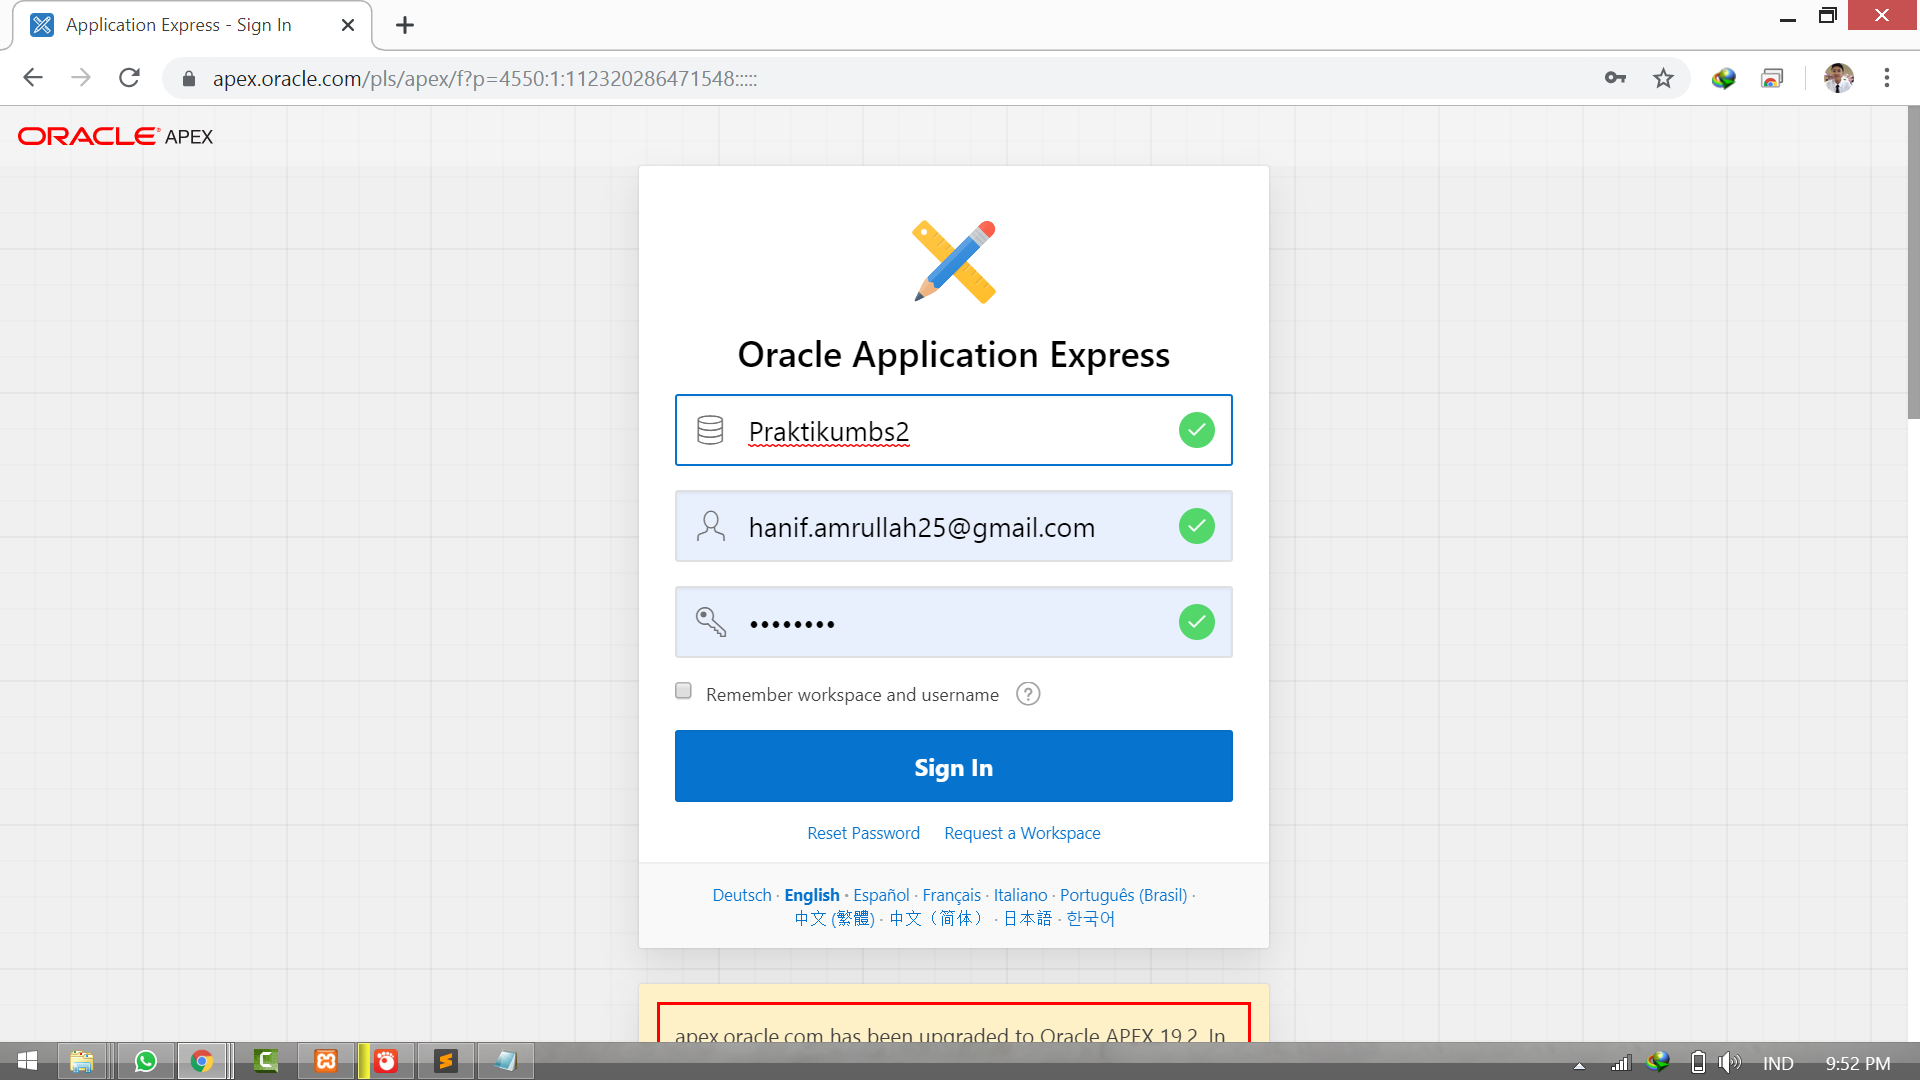
\includegraphics[scale=0.5]{figures/1.png}
        \caption{Create}
        \label{penanda}
    \end{figure}
\newline
    \item  lalu create
\newline
    \item  Setelah itu unggah file dalam bentuk csv,xlxs,xml atau json .
    \newline
    \begin{figure}[!htbp]
        \centering
        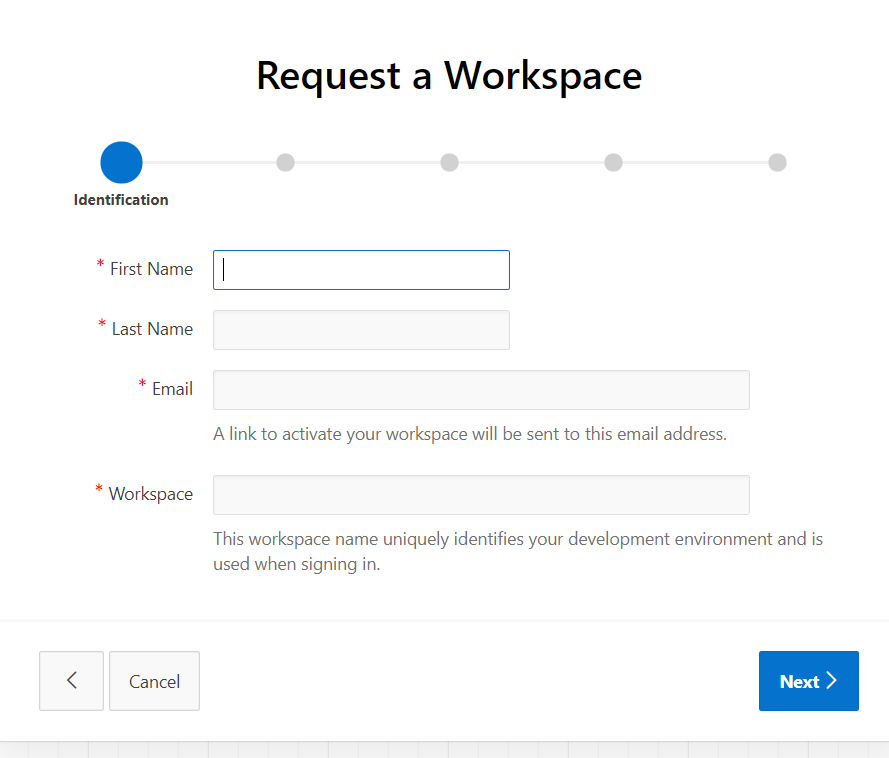
\includegraphics[scale=0.5]{figures/3.png}
        \caption{Memasukan file}
        \label{penanda}
    \end{figure}
\newline
    \item  Kemudian pilih file data excel yang telah dibuat dalam bentuk xlsx
\newline
    \item  Buat tabel dengan memasukkan nama tabel disini saya membuat tabel Mahasiswa terlebih dahulu .
    \newline
    \begin{figure}[!htbp]
        \centering
        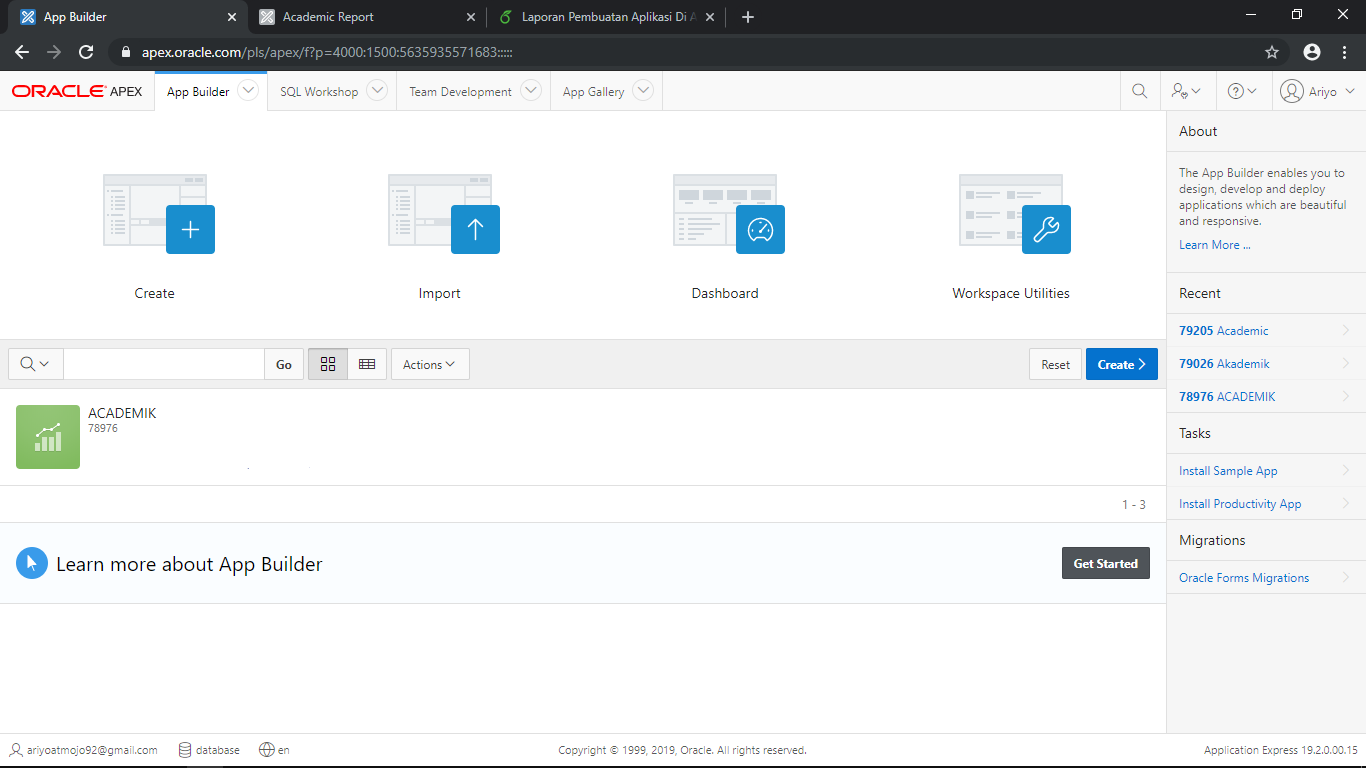
\includegraphics[scale=0.5]{figures/4.png}
        \caption{Membuat nama tabel Mahasiswa}
        \label{fig:my_label}
    \end{figure}
\newline
    \item Klik configure untuk mengecek apakah tabel dari data excel sudah benar atau tidak 
\newline
    \item  Lalu scroll kebawah sehingga keluar daftar nama mahasiswa yang berada pada file excel kemudian klik load data 
\newline
    \item Kemudia klik X untuk membuat tabel berikutnya , lakukan seperti perintah yang diatas lagi . selanjutnya membuat tabel dosen 
\newline
    \begin{figure}[!htbp]
        \centering
        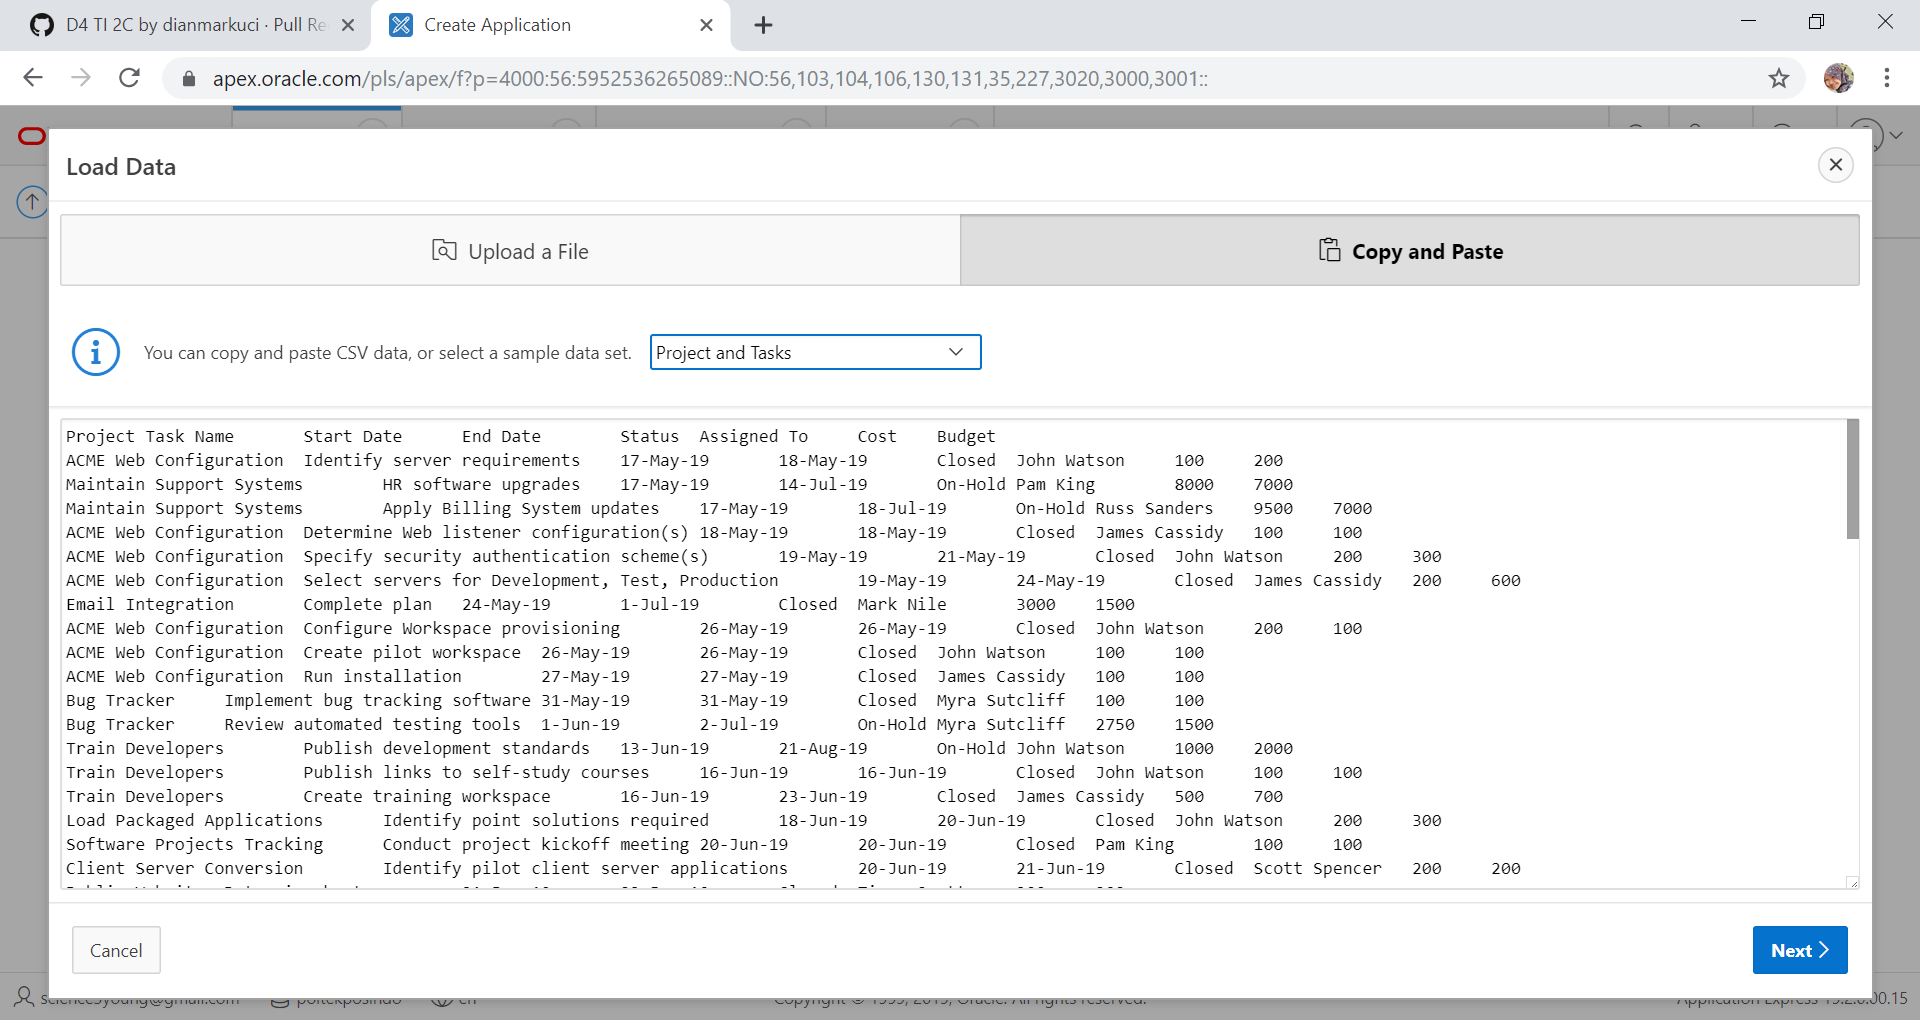
\includegraphics[scale=0.5]{figures/7.png}
        \caption{Membuat nama tabel dosen}
        \label{fig:my_label}
    \end{figure}
\newline
    \item Lalu configure dan klik load data , lalu klik X untuk keluar .
    \newline
    \item Kemudian membuat tabel Kuliah .
    \begin{figure}[!htbp]
        \centering
        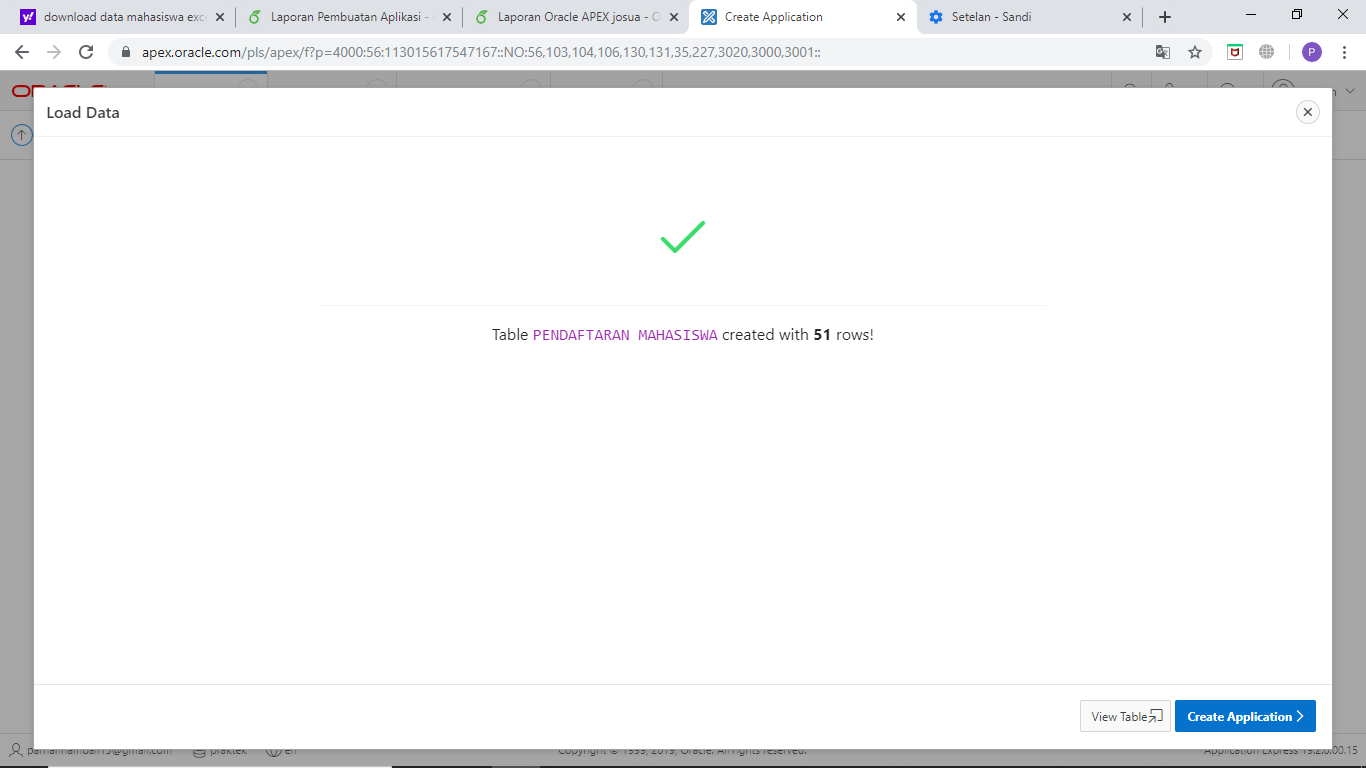
\includegraphics[scale=0.5]{figures/8.png}
        \caption{Membuat nama tabel kuliah}
        \label{fig:my_label}
    \end{figure}
    \newline
    \item Lakukan lagi perintah seperti diatas sampai semua tabel selesai dibuat . setelah tabel kuliah membuat tabel jadwal .
    \newline
    \begin{figure}[!htbp]
        \centering
        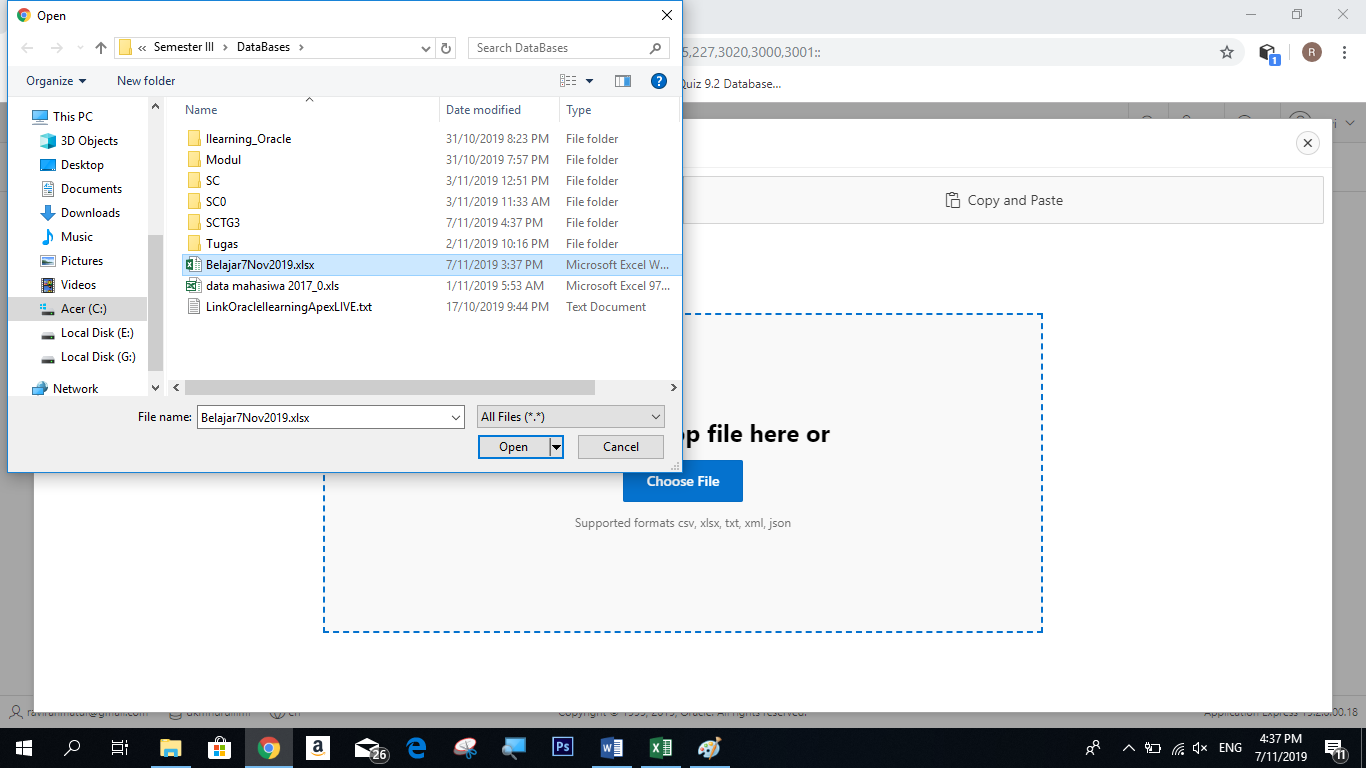
\includegraphics[scale=0.5]{figures/9.png}
        \caption{Membuat nama tabel jadwal}
        \label{fig:my_label}
    \end{figure}
    \newline
    \item Membuat tabel nilai . 
    \newline
    \begin{figure}[!htbp]
        \centering
        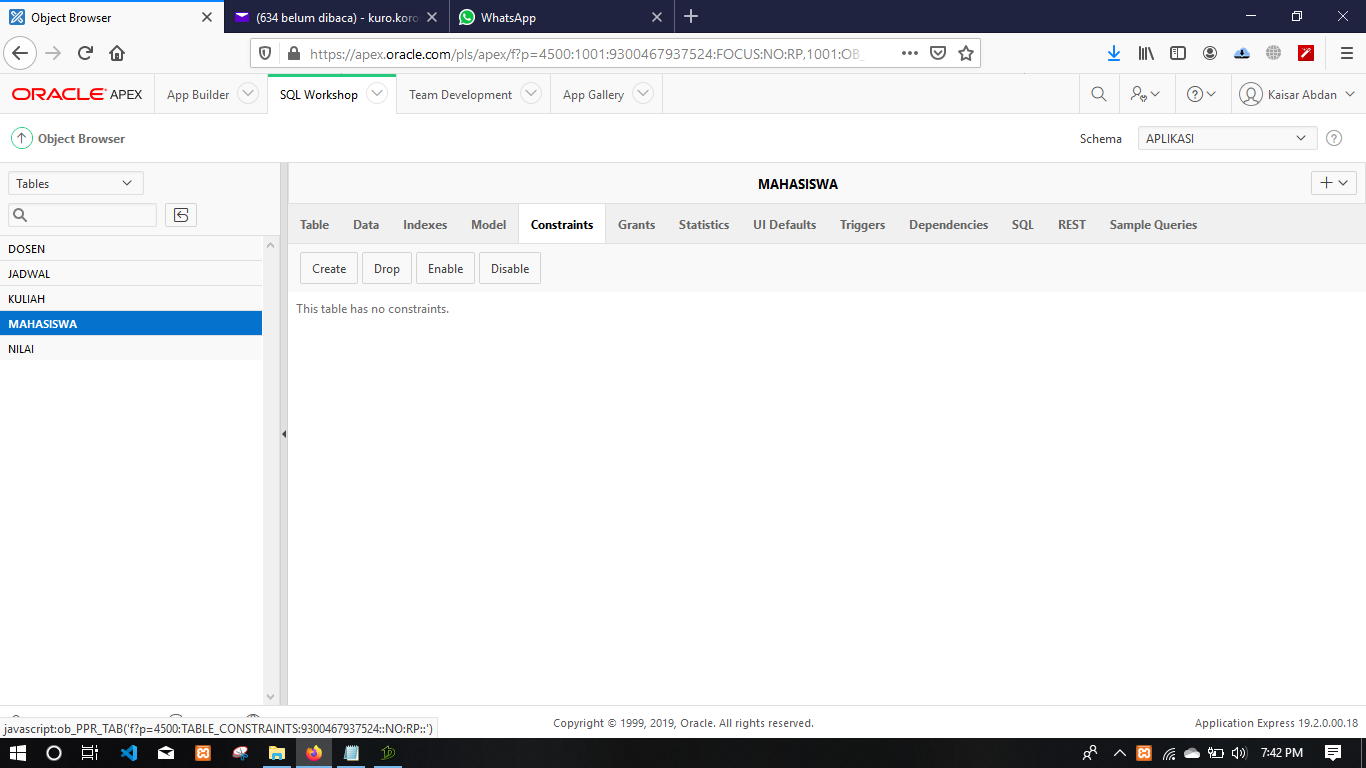
\includegraphics[scale=0.5]{figures/10.png}
        \caption{Mmebuat nama tabel nilai}
        \label{fig:my_label}
    \end{figure}
    \newline
    \item  Tampilan selanjutnya adalah create lalu hapus ID disetiap tabel .
\newline
\begin{figure}[!htbp]
    \centering
    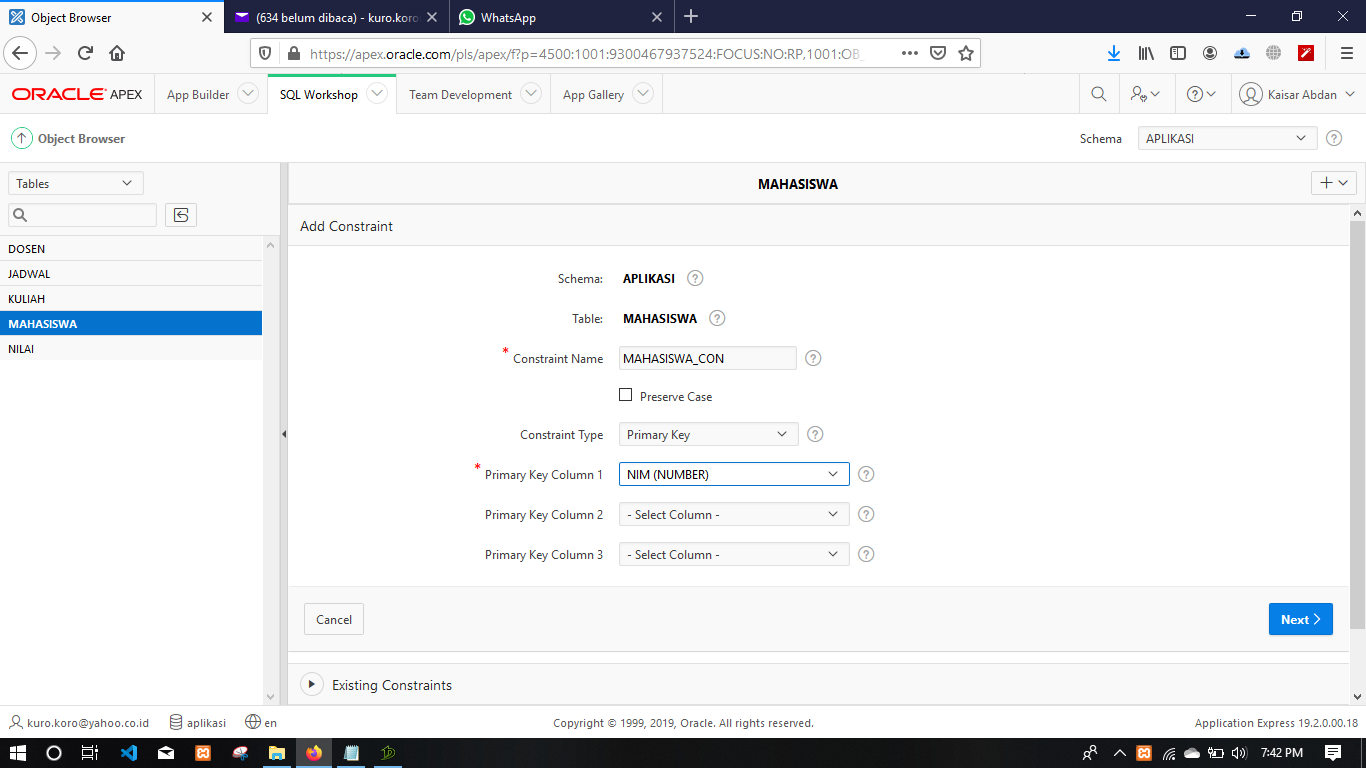
\includegraphics[scale=0.5]{figures/12.png}
    \caption{Menghapus ID}
    \label{fig:my_label}
\end{figure}
\newline
\item Lalu ubah setaip tabel ke primary dan foreign key , pertama kita ubah terlebih dahulu yang primary seperti Dosen , Mahasiswa dan kuliah sedangan jadwal dan nilai kita ubah ke foreign key .
\newline
\begin{figure}[!htbp]
    \centering
    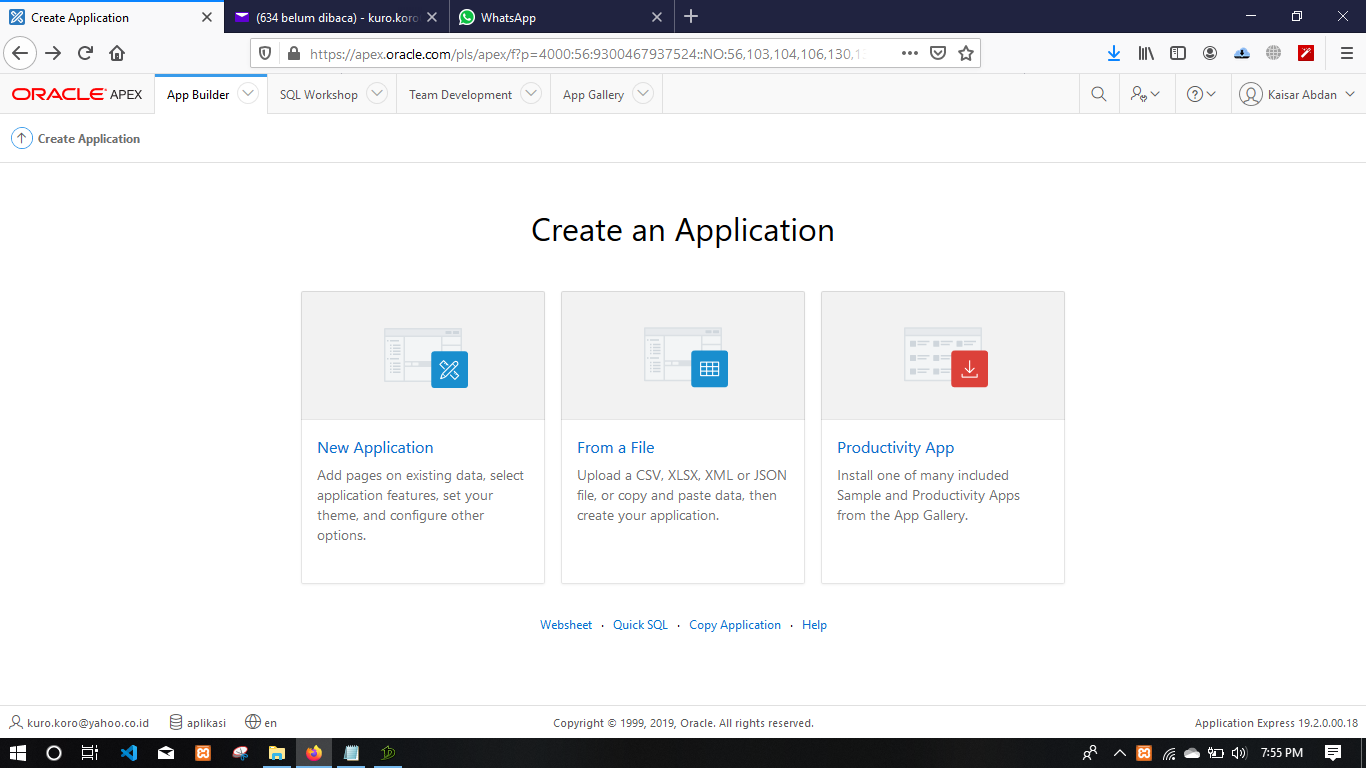
\includegraphics[scale=0.3]{figures/20.png}
    \caption{Mengubah tabel menjadi primary dan foreign key}
    \label{fig:my_label}
\end{figure}
\newline
\item Setelah itu kita buka app builder dan create .
\newline
\begin{figure}[!htbp]
    \centering
    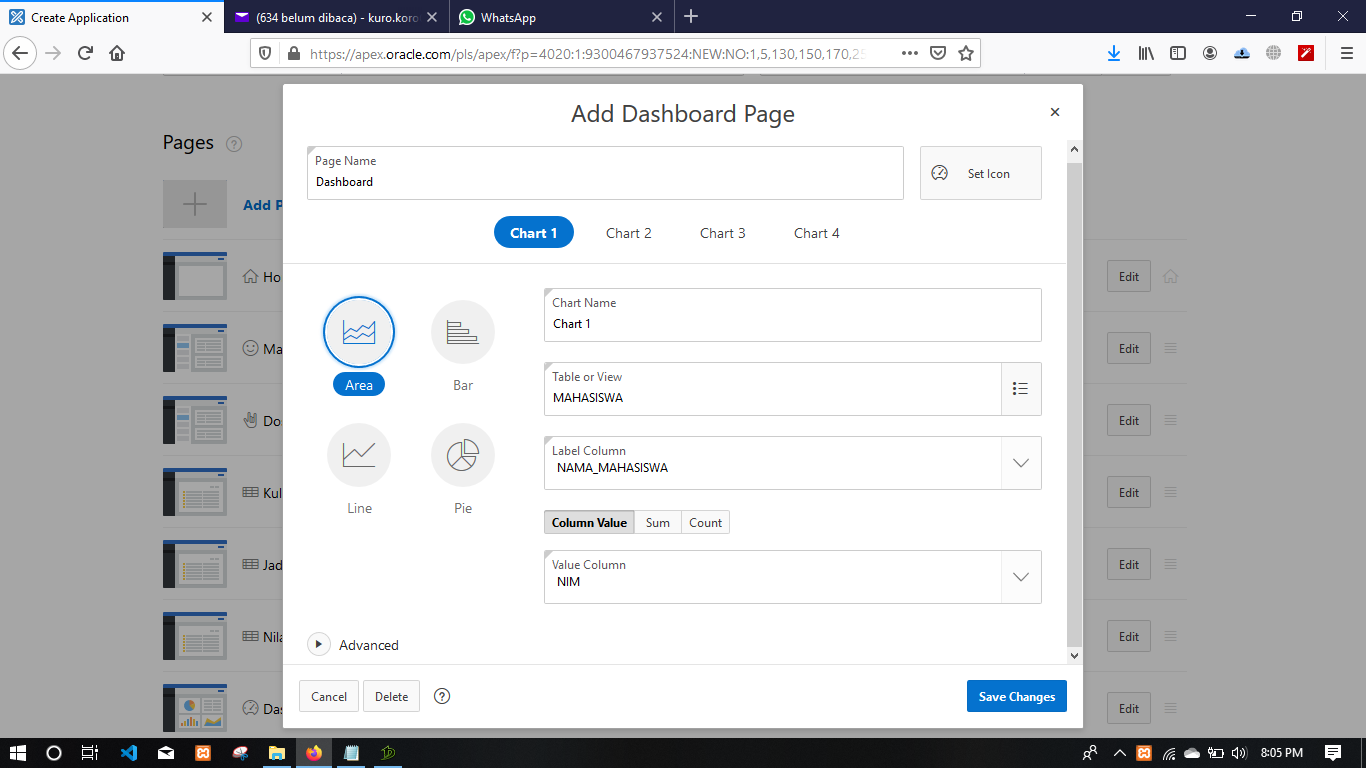
\includegraphics[scale=0.5]{figures/24.png}
    \caption{App Builder}
    \label{fig:my_label}
\end{figure}
\newline
\item Kemudian add page untuk memilih fitur apa saja yang mau digunakan . 
\newline
\begin{figure}[!htbp]
    \centering
    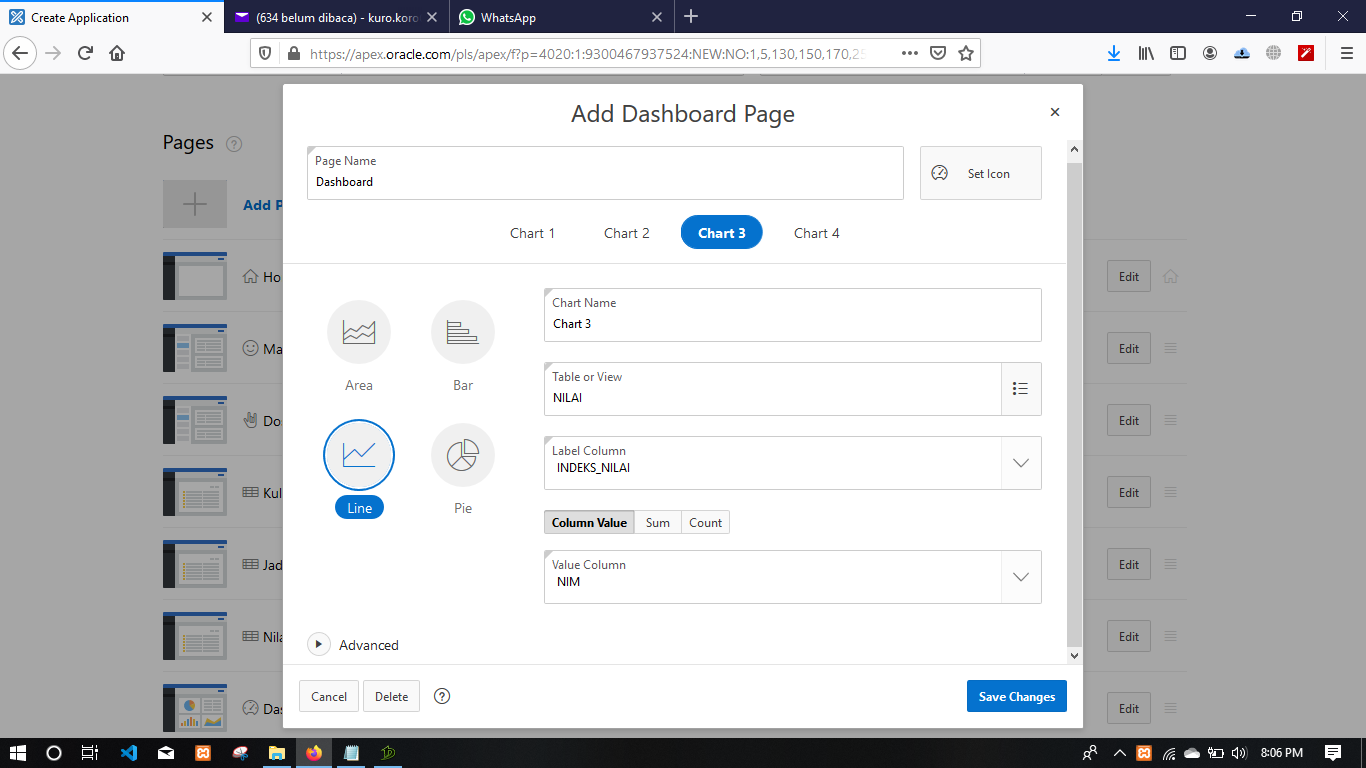
\includegraphics[scale=0.5]{figures/26.png}
    \caption{Add page}
    \label{fig:my_label}
\end{figure}
\newline
\item Setelah itu Create An application 
\newline
\begin{figure}[!htbp]
    \centering
    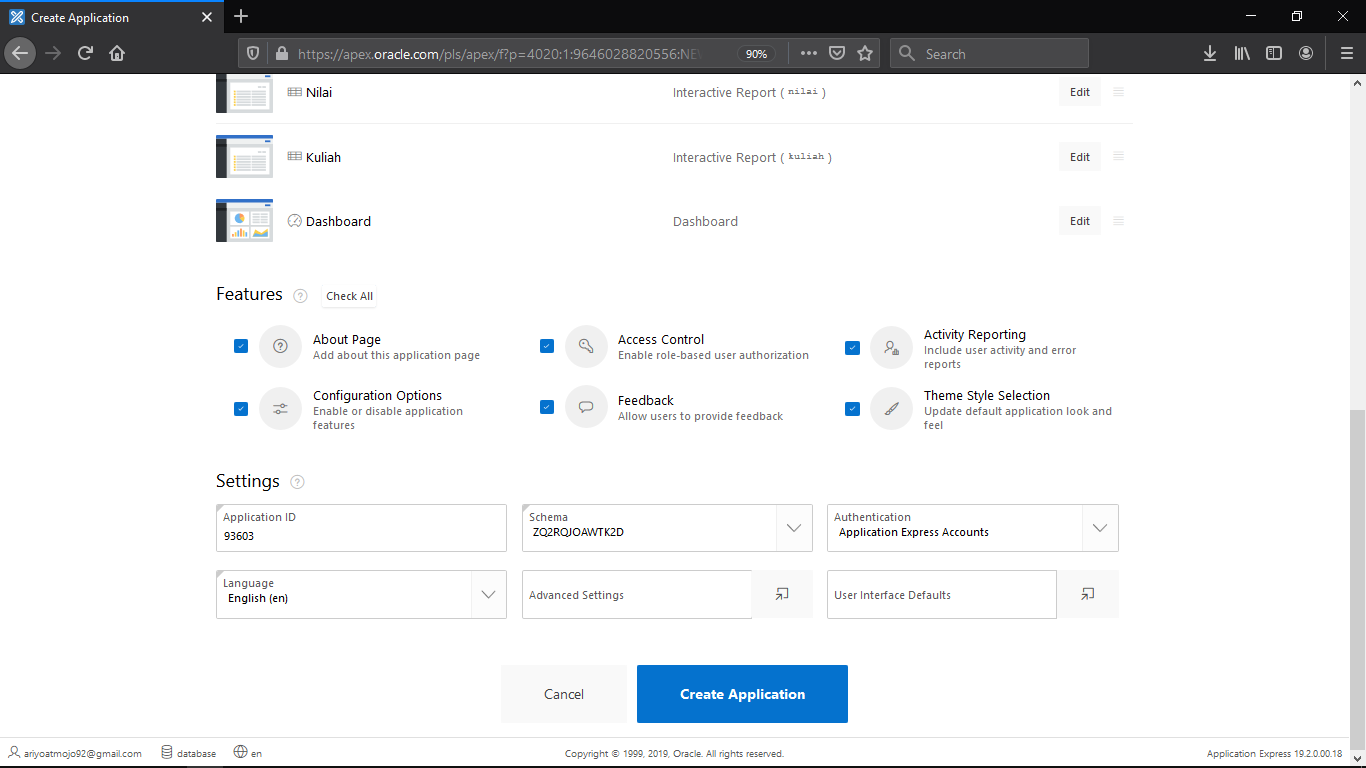
\includegraphics[scale=0.5]{figures/38.png}
    \caption{Create An Application}
    \label{fig:my_label}
\end{figure}
\newline
    \item  lalu klik check all
\newline
    \item  Maka selanjunya jalankan aplikasi dengan mengklik run application
\newline
\begin{figure}[!htbp]
    \centering
    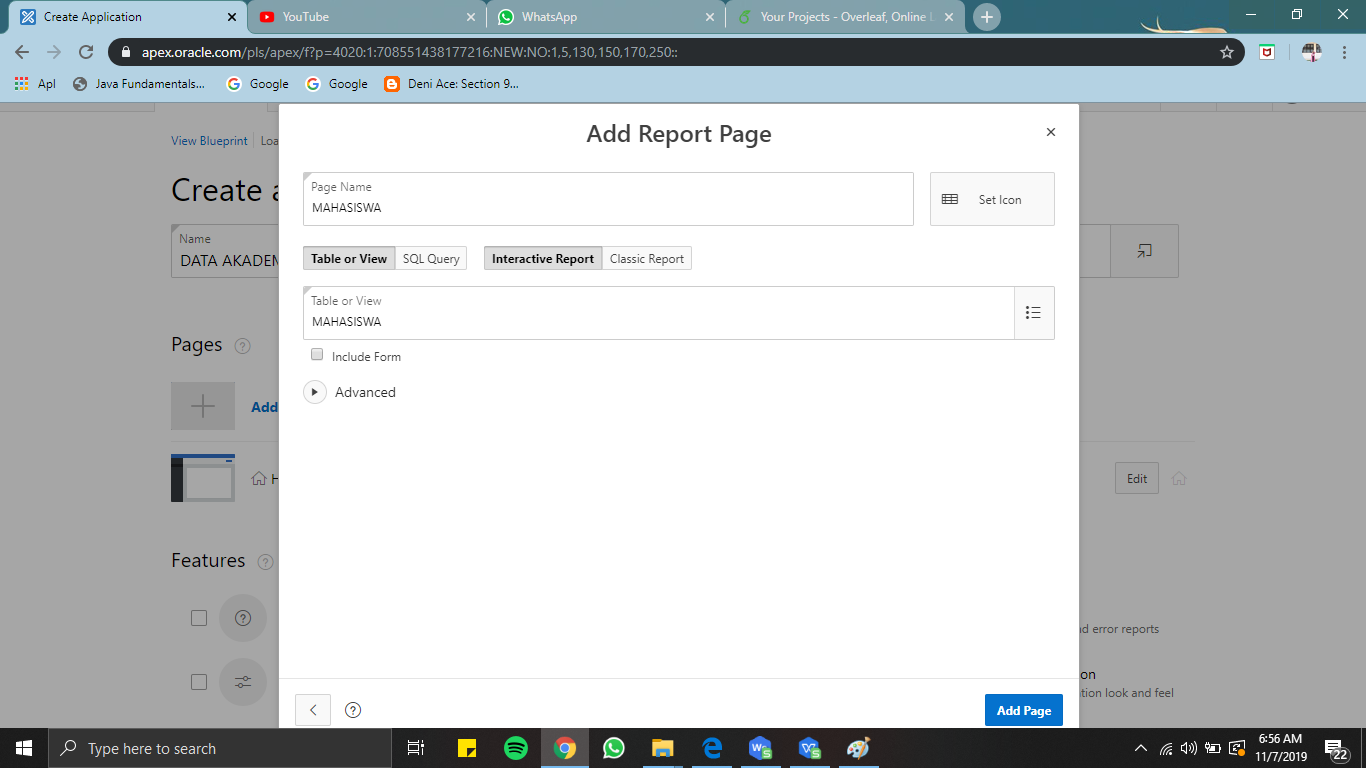
\includegraphics[scale=0.5]{figures/40.png}
    \caption{Run Application}
    \label{fig:my_label}
\end{figure}
\newline

\item Lalu masukkan email dan password untuk masuk ke aplikasi nya . 
\newline
\begin{figure}[!htbp]
    \centering
    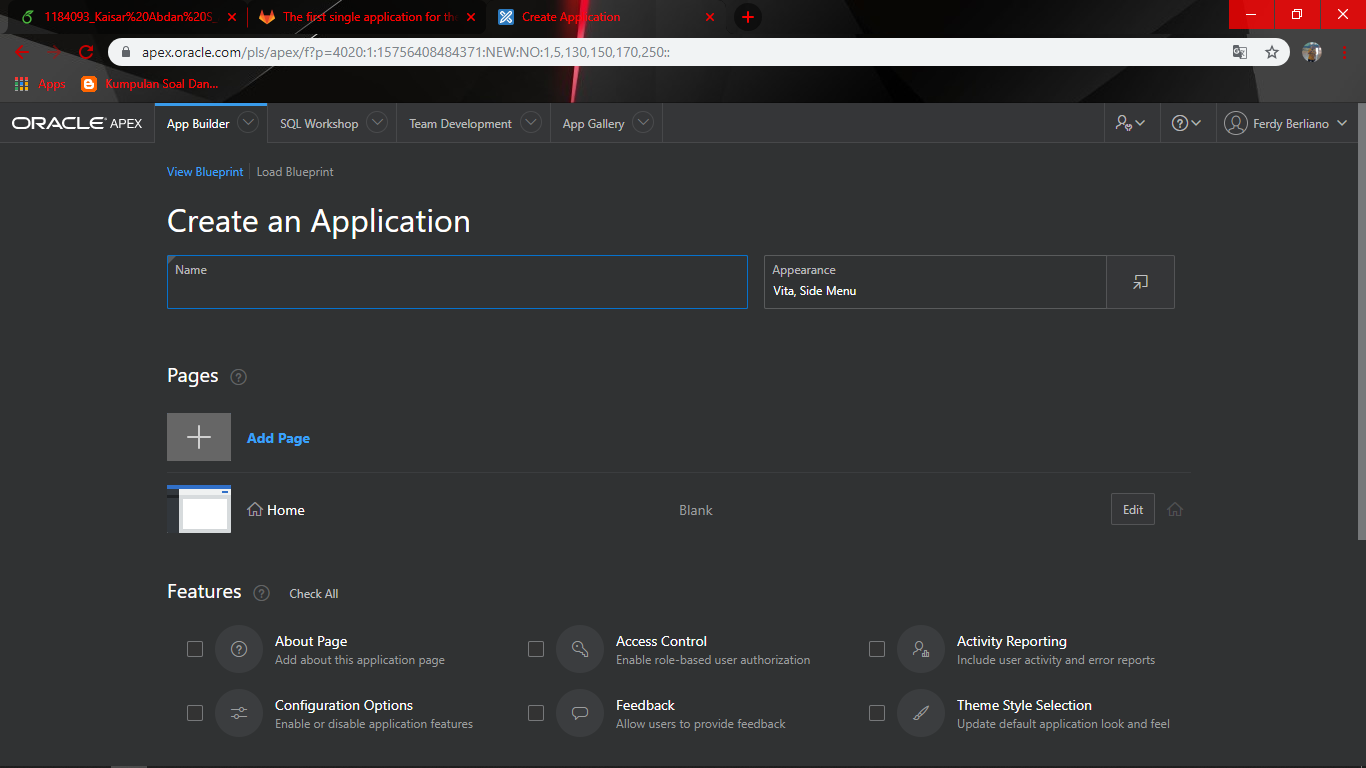
\includegraphics[scale=0.7]{figures/41.png}
    \caption{Sign in}
    \label{fig:my_label}
\end{figure}
\newline
    \item  Maka akan muncul aplikasi sistem sederhana akademik 
\newline
\begin{figure}[!htbp]
    \centering
    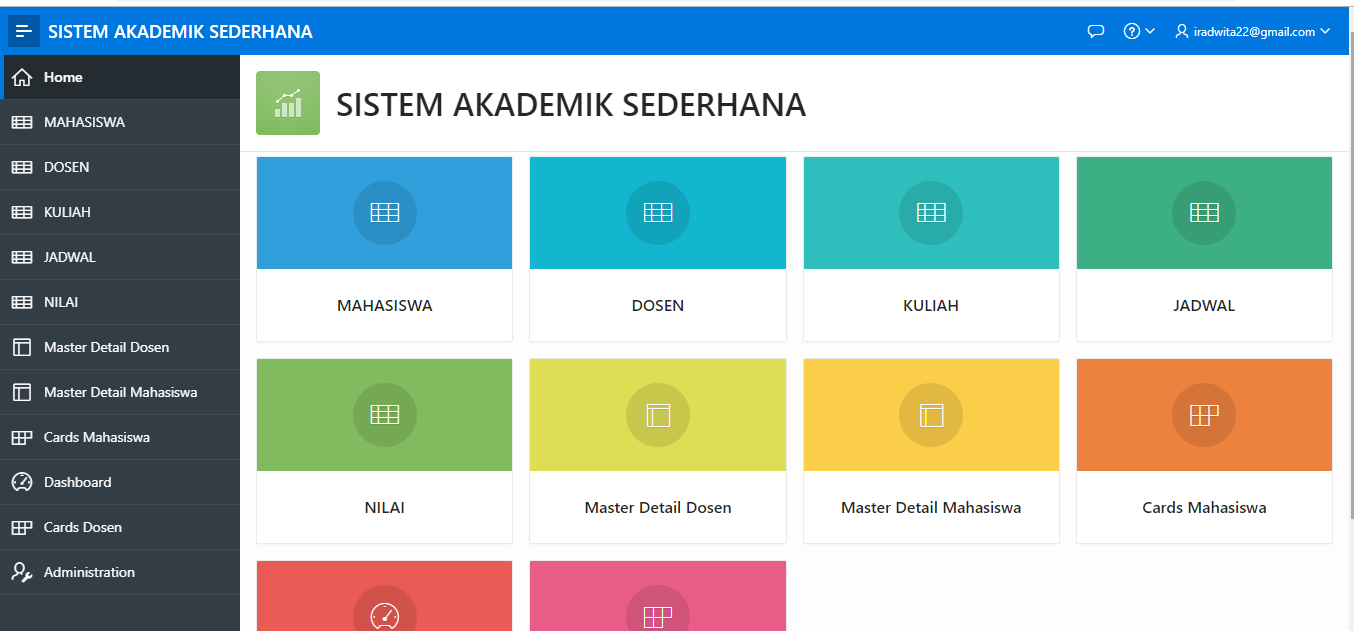
\includegraphics[scale=0.3]{figures/42.png}
    \caption{Aplikasi Sistem Akademik Sederhana}
    \label{fig:my_label}
\end{figure}
\newline
    \item  Aplikasi akademik selesai dibuat .
\end{enumerate}

link : https://apex.oracle.com/pls/apex/f?p=76816:LOGIN_DESKTOP:711761223598218:::::

Email : IRADWITA22@GMAIL.COM

Password :#Ira1234






\begin{enumerate}


\end{enumerate}


%now enable appendix numbering format and include any appendices
%\appendix
%\chapter{Form Penilaian Jurnal}

gambar \ref{form1} dan \ref{form2} merupakan contoh bagaimana reviewer menilai jurnal kita. 
\begin{figure}[ht]
      \centerline{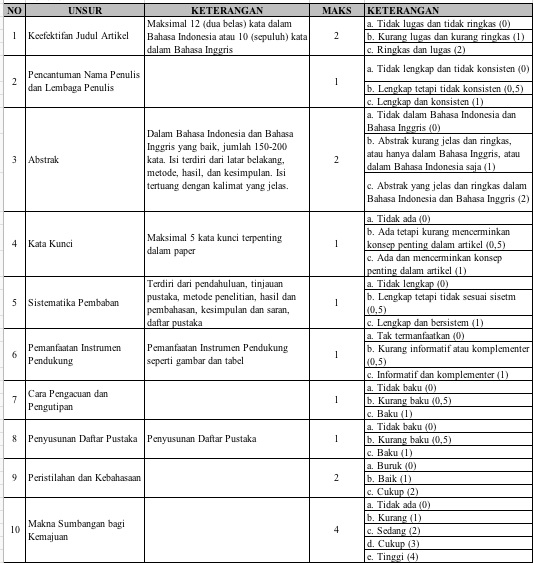
\includegraphics[width=1\textwidth]
      {figures/form1}}
      \caption{Form nilai bagian 1.}
      \label{form1}
      \end{figure}

	\begin{figure}[ht]
	      \centerline{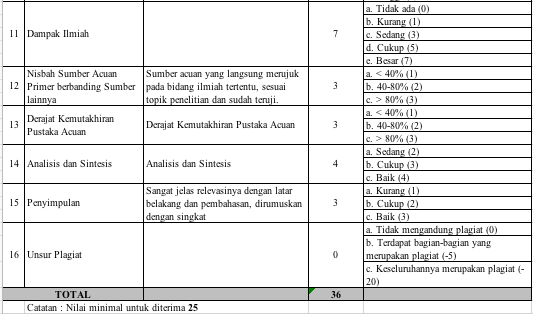
\includegraphics[width=1\textwidth]
	      {figures/form2}}
	      \caption{form nilai bagian 2.}
	      \label{form2}
	      \end{figure}

%\chapter{FAQ}

M : Kalo Intership II atau TA harus buat aplikasi ?
D : Ga harus buat aplikasi tapi harus ngoding

M : Pa saya bingung mau ngapain, saya juga bingung mau presentasi apa?
D : Makanya baca de, buka jurnal topik `ganteng' nah kamu baca dulu sehari 5 kali ya, 4 hari udah 20 tuh. Bingung itu tanda kurang wawasan alias kurang baca.

M : Pa saya sudah cari jurnal terindeks scopus tapi ga nemu.
D : Kamu punya mata de? coba dicolok dulu. Kamu udah lakuin apa aja? tolong di list laporkan ke grup Tingkat Akhir. Tinggal buka google scholar klik dari tahun 2014, cek nama jurnalnya di scimagojr.com beres.

M : Pa saya belum dapat tempat intership, jadi ga tau mau presentasi apa?
D : kamu kok ga nyambung, yang dipresentasikan itu yang kamu baca bukan yang akan kamu lakukan.

M : Pa ini jurnal harus yang terindex scopus ga bisa yang lain ?
D : Index scopus menandakan artikel tersebut dalam standar semantik yang mudah dipahami dan dibaca serta bukan artikel asal jadi. Jika diluar scopus biasanya lebih sukar untuk dibaca dan dipahami karena tidak adanya proses review yang baik dan benar terhadap artikel.

M : Pa saya tidak mengerti
D : Coba lihat standar alasan

M : Pa saya bingung
D : Coba lihat standar alasan

M : Pa saya sibuk
D : Mbahmu....

M : Pa saya ganteng
D : Ndasmu....

M : Pa saya kece
D : wes karepmu lah....


Biasanya anda memiliki alasan tertentu jika menghadapi kendala saat proses bimbingan, disini saya akan melakukan standar alasan agar persepsi yang diterima sama dan tidak salah kaprah. Penggunaan kata alasan tersebut antara lain :

1. Tidak Mengerti : anda boleh menggunakan alasan ini jika anda sudah melakukan tahapan membaca dan meresumekan 15 jurnal. Sudah mencoba dan mempraktekkan teorinya dengan mencari di youtube dan google minimal 6 jam sehari selama 3 hari berturut-turut.

2. Bingung : anda boleh mengatakan alasan bingung setelah maksimal dalam berusaha menyelesaikan tugas bimbingan dari dosen(sudah dilakukan semua). Anda belum bisa mengatakan alasan bingung jika anda masih belum menyelesaikan tugas bimbingan dan poin nomor 1 diatas. Setelah anda menyelesaikan tugas bimbingan secara maksimal dan tahap 1 poin diatas, tapi anda masih tetap bingung maka anda boleh memakai alasan ini.

%next line adds the Bibliography to the contents page
\addcontentsline{toc}{chapter}{Daftar Pustaka}
%uncomment next line to change bibliography name to references
%\renewcommand{\bibname}{References}
        %use a bibtex bibliography file refs.bib
\bibliographystyle{plain}  %use the plain bibliography style

\end{document}

